\chapter{Introduction \nd Theoretical Overview}

The field of particle physics is rooted in the aspiration to address some of the most fundamental questions of the universe that we live in, \ie, 
what are we and everything around us made up of? The human quest to understand the most fundamental building blocks of the universe and their 
interactions has a long history. The ancient Indians believed the universe to be made of five basic elements: air, earth, fire, space, and water. 
Similar ideas also prevailed in other civilizations as well. In 6th century B.C. an Indian philosopher named Kanaada espoused a form of atomism and 
postulated that all objects in the physical universe were reducible to a finite number of atoms, which he called ``anu''. The Greek philosophers 
Leucippe and his disciple Democritus in 5th century B.C. hypothesized that everything on earth was composed of small indivisible entities, called 
``the atomos", the Greek word for indivisible. This understanding has evolved from its roots in natural philosophy and metaphysics into an area of 
natural science in which experiments attempt to confirm or reject theories that describe the nature of elementary constituents. The picture of these 
building blocks has changed over the period of time and has led to the development of the ``Standard Model (\gls{SM})'' of particle physics~\cite{Glashow:1961tr, Salam:1964ry, Weinberg:1967tq}. In the last few decades, physics at high energies ($\sim$GeV/TeV) has proven to be an efficient way 
to build and test the SM. In high energy collider experiments, the fundamental idea is to steer two accelerated beams of particles together in opposite 
directions and study the properties of the remnant particles produced in the collision.

In this chapter, the theoretical framework of the SM, used to describe the elementary particles and their interactions, is outlined 
briefly. In addition, the motivation for the search of physics beyond the SM and a brief introduction to the physics of compositeness is also
presented.  Chapter 2 describes the Large Hadron Collider (\gls{LHC}), the machine which produces proton-proton (pp) collisions, and the Compact Muon
Solenoid (\gls{CMS}) detector, the instrument which records these interactions. While Chapter 3 discusses the event generation and simulation for 
signal and background processes, Chapter 4 describes the reconstruction of the physics objects used in the analyses. Chapter 5 describes, in detail, 
the physics analysis used for the search of excited quarks in the \gamjet final state and Chapter 6 summarizes the results of the analysis.

\section{The Standard Model of Particle Physics}
The modern era of particle physics began at the end of the 19$^{th}$ century with the discovery of the first subatomic particle, 
the electron~\cite{ElectronDiscovery}, by J. J. Thomson in 1897, when he observed bending of the cathode rays in the presence of a magnetic field. 
The chemists and physicists continued their work for several decades to understand the structure of the atom. In 1911, Rutherford gave the concept 
of nucleus~\cite{Rutherford:1911zz,Rutherford1913} by analyzing the data of Geiger and Marsden on the scattering of $\alpha-$particles against a 
thin gold foil. He showed that atoms consist of a compact positively charged nucleus and a cloud of negative charge composed of electrons. Observations 
by Thomson and Rutherford led N. Bohr, in 1914, to propose a theory of atomic structure based on quantum ideas~\cite{Bohr1913}. However, the 
understanding of the composition of the atom only became complete with the discovery of neutrons by Chadwick in 1932~\cite{Chadwick1932}. It was 
thus confirmed, by early 1930s, that ordinary matter consists of three particles: electrons, protons, and neutrons. 

Around the same period, in 1900, M. Planck proposed that electromagnetic radiation comes in packets as quanta of energy but gave no explanation
for quantization, which was later given by Albert Einstein in 1905 using the theory of photoelectric effect~\cite{Einstein:1905ve}. The quanta of 
electromagnetic radiation was later termed as ``photon'' by Gilbert N. Lewis in 1926. The discovery of Compton effect by Arthur Holly Compton in 1923
confirmed the particle nature of the photons~\cite{Compton:1923zz}. A. Einstein, in 1905, introduced a theory of special relativity, that took
several years to be accepted, while Paul Dirac, in 1927, combined it with quantum mechanics to a form a single theory, known as ``quantum field 
theory''~\cite{Dirac1927}. Dirac used quantum field theory to describe the behaviour of free electrons.
Dirac's equation though appeared to be correct, had negative energy solutions, that could only be explained by the presence of a particle with mass 
same as that of an electron but opposite in charge. The discovery of positron (anti-electron) in 1933 by Carl Anderson~\cite{Anderson:1933mb} was 
a triumph of Dirac's theory. This was the first observation of an anti-particle.

Another astonishing observation seen in the same period was the energy spectrum of electrons in nuclear $\beta$ decay. Assuming the decay of 
a nucleus into a lighter nuclei and an electron, the energy of the electron could be explicitly predicted by its kinematics. However, it was
observed that the energy spectrum of the electrons was softer and broader than the energies predicted. The effect was explained by Pauli in 
1930 by introducing an invisible particle that carried away the missing energy and momentum, and which was termed neutrino ($\nu$) in 1932 by 
Enrico Fermi. As this process can be explained neither by electromagnetic nor by strong interactions, Fermi in 1934 put forth a theory of 
$\beta$ decay~\cite{Fermi1934} that introduced the theory of weak interactions. The neutrinos were experimentally observed for the first time 
in 1956 by Cowan and Reines~\cite{Cowan:1992xc}. They studied the inverse $\beta$ decay process $\bar{\nu}+p^{+}\to{n}+e^{-}$ in a large tank of 
cadmium enriched water at the Savannah river nuclear reactor that gave evidence for anti-neutrino (at that time thought to be neutrino) existence 
by identifying the positrons. 

One question that bothered everyone at that time (1930s) was what binds the nucleus together? Confining several positive charges together into a
small region ($1\unit{fm}=10^{-15}\unit{m}$) results in a strong repulsive electrostatic force. If nuclei are to be stable then the protons
need to be bound together by a powerful force. This force was called ``strong force''. Hideki Yukawa in 1934 combined quantum theory and
relativity to describe nuclear interaction among nucleons via exchange of a particle called meson~\cite{Yukawa:1935xg}, later termed
as ``pions''. Yukawa postulated that the mass of these mesons must be $\sim300$ times the mass of electron. Anderson and Neddermeyer
in 1937~\cite{Neddermeyer:1937md} searched for this particle in cosmic rays and found a particle with mass $\sim200$ times that of electron mass, 
which turned out to be a different particle, later called the muon ($\mu$). The muon is a particle with quantum numbers same as that of an electron 
but with larger mass. Eventually the pion was discovered by Cecil Powell in cosmic ray experiments in 1947~\cite{Lattes:1947mx}.

The period after 1940's saw the beginning of particle physics as a distinct field of study with the pioneering work of 
Feynman~\cite{Feynman:1948ur,Feynman:1948km,Feynman:1949hz}, Schwinger~\cite{Schwinger:1948iu,Schwinger:1948yk}, and Tomonaga~\cite{Tomonaga:1948zz},
who together, developed the theory of Quantum Electrodynamics (\gls{QED})~\cite{Dyson:1949bp} which explained electromagnetic processes at a basic 
level in terms of the exchange of photons. The decades of 1940's and 1950's saw a number of particles being discovered in scattering experiments. In 
1947, a particle called the Kaon, having a long lifetime was discovered by Rochester and Butler~\cite{Rochester:1947mi}. Another particle with 
similar property, called $\Lambda$, was observed by Hopper and Biswas in 1950~\cite{PhysRev.80.1099}. These strange particles were produced copiously 
and quickly but decayed very slowly. These were later assigned a new quantum number, Strangeness, by Gell-Mann and Nishijima. With advances in the 
particle physics experiments, in subsequent years more and more new particles were found. In an attempt of arrange these particles they were classified 
into leptons (light weight), mesons (medium weight) and baryons (heavy weight). The electon, muon, and the neutrino belonged to the species of leptons. 
Further to this, Murray Gell-Mann organized the hadrons (mesons and baryons) based on charge and strangeness into the famous ``Eightfold way'', which 
led to the prediction of $\Omega^{-}$ with a strangeness quantum number of -3.

In 1964, Gell-Mann and Zweig~\cite{GellMann:1964nj,Zweig:570209} proposed the `quark model' according to which the hadrons have sub-structure and are
made up of fundamental particles called `quarks'. These proposed quarks were to be of three types or flavors, namely, up ($u$), down, ($d$),
and strange ($s$). According to this model, baryons consist of three quarks while the mesons are made up of a quark and an anti-quark pair.
 The weakness for this model was that no free quark had been observed by then and as per Pauli's exclusion principle three identical quarks (fermions) 
cannot co-exist together, which led to the introduction of a new quantum number, `color'. The quark model required hadrons to be colorless entity and 
didn't allow quarks to exist in free state. A major triumph for the quark model was the discovery of already predicted $\Omega^{-}$ with known
quantum numbers at the Brookhaven National Laboratory (BNL)~\cite{Barnes:1964pd}. In 1967, experiments which had beam of electrons striking nuclear 
targets (or $e-p$ interactions) \ie, scattering of electron off protons at the experiment at \gls{SLAC} showed the existence of substructure in the 
proton, in a manner similar to the way scattering experiments of Rutherford proved the existence of substructure in the atom.

The elementary particles known to physicists by this time comprised of three quarks, $u$, $d$, and $s$, four leptons, $e^{-}, \nu_{e}, \mu^{-}$ 
and $\nu_{\mu}$ and a boson, called photon. The apparent asymmetry between the number of leptons and quarks, in 1964 led Glashow and 
Bjorken~\cite{Bjorken:1964gz} to predict that there might exist a fourth quark  and they named it `charm'. Later in 1970, Glashow, 
Iliopoulos and Maiani~\cite{Glashow:1970gm} classified particles so that there is symmetry between leptons [($e,\nu_{e}$),($\mu, \nu_{\mu}$)] 
and quarks [($u,d$),($s,c$)]. They introduced a new quantum number, weak isospin which need to be conserved for weak interactions and also 
suggested additional $c$ quark that was not yet discovered. In 1974, two seperate experimental groups, one led by S.C.C. Ting at the \gls{BNL_AGS}
proton synchrotron and other lead by B. Richter at SLAC/\gls{SPEAR} $e^{+}e^{-}$ collider independently observed a narrow resonance of the $c\bar{c}$ 
bound state ($J/\psi$ particle)~\cite{Aubert:1974js,Augustin:1974xw}. The generational structure for leptons got extended with the discovery of 
$tau\;(\tau)$ lepton by M. Perl et. al. at SLAC/SPEAR in 1975~\cite{Perl:1975bf}. This discovery again led to the asymmetry in the number of 
leptons and baryons and made physicists to search for a new family of quarks. Two years later in 1977, the observation of $b\bar{b}$ bound state, 
$Upsilon (\Upsilon)$ particle by Leon Lederman at Fermilab added new beauty/bottom ($b$) quark~\cite{Herb:1977ek} to the family of quarks. 
After a wait of 18 years, the last in the family of quarks the top $(t)$ quark was observed in 1995 at the \gls{CDF}~\cite{Abe:1995hr} and 
\gls{D0}~\cite{Abachi:1995iq} experiements at Fermilab.

Discovery of hadron sub-structure suggested a new fundamental explanation of strong nuclear forces to replace Yukawa's meson mediation theory. A
new theory, predicting a new particle, gluon, mediating these strong interactions was proposed during this period. The gluon was discovered,
when a three-jet event was observerd in electron positron collision at TASSO experiment~\cite{Gluons1979} at PETRA collider in 1979. E. Fermi 
treated theory of weak interactions as contact interactions without  introduction of any mediating particles, which proved to be very effective at 
low energies, however the resuls from Gargamelle experiments at CERN~\cite{Hasert:1973ff} differed with the theory at higher energies. 
S. Glashow~\cite{Glashow:1961tr}, A. Salam~\cite{Salam:1964ry}, and S. Weinberg~\cite{Weinberg:1967tq} proposed a 
theory of weak interactions which unified electrodynamics and weak interactions and demanded the existence of gauge bosons to mediate these 
interactions. One concern for this electroweak theory was that the $W/Z$ bosons had to be massless for the theory to be consistent, while they needed
to be heavy for interactions to be weak. The mass of these bosons was explained by the spontaneous symmetry breaking of weak 
interactions via Higgs mechanism proposed by Higgs~\cite{Higgs:1964ia,Higgs:1964pj,Higgs:1966ev}, Englert $\&$ Brout~\cite{Englert:1964et}, Guralnik, 
Kibble, $\&$ Hagen~\cite{Guralnik:1964eu} in mid 1960's. The Higgs mechanism predicted a new particle, later called the Higgs boson. The charged weak 
bosons, $W^{\pm}$~\cite{Arnison:1983rp,Banner:1983jy} and neutral weak boson, $Z$~\cite{Arnison:1983mk,Arnison:1983zy, Bagnaia:1983zx} were later 
discovered in 1983 by the UA1 and UA2 collaborations in $p\bar{p}$ collisions at \gls{CERN}. 

The observation of a new boson with properties similar to that of a Higgs boson by the \gls{ATLAS}~\cite{Aad:2012tfa} and the 
CMS~\cite{Chatrchyan:2012xdj} collaborations with a mass of $\sim125\unit{GeV}$ was an important milestone in the decades long 
hunt for understanding of the mechanism of electroweak symmetry breaking. In light of this observation at the LHC, the 2013 Nobel 
Prize in Physics was awarded to Francois Englert and Peter Higgs for the development  of spontaneously broken local gauge theories 
and theoretical insights on the origin of mass.

The properties of the Higgs boson have been extensively studied by the ATLAS~\cite{ATLAS:2014yka} and the CMS~\cite{CMS:yva} collaborations. 
The mass of the Higgs particle has been measured to be $m_{H}=125.5\pm0.2(\text{stat})^{+0.5}_{-0.6}(\text{sys})\unit{GeV}$/c$^{2}$ by ATLAS
 with a combined signal strength of $\mu=1.30\pm0.12(\text{stat})^{+0.14}_{-0.11}(\text{sys})$~\cite{ATLAS:2014yka} where $\mu=\sigma/\sigma_{SM}$
and $m_{H}=125.03\pm0.27(\text{stat})\pm0.15(\text{sys})\unit{GeV}$/c$^{2}$ by CMS with a combined signal strength of $\mu=1.00\pm0.09(\text{stat})
\pm0.07(\text{sys})$~\cite{CMS:yva}.

According to our present knowledge, leptons and quarks are fundamental particles, i.e., they are point-like and do not appear to have 
sub-structures. Our present understanding of the elementary particles and their interactions is encapsulated in the SM of particle physics.

\subsection{Fundamental Particles}
The SM is the theoretical basis of modern particle physics which cohesively binds the amalgamantion of last $60-70$ years of data on
elementary particles and their interactions. Summarizing the historical introduction, the SM in its present state, consists of `matter particles':
 fundamental units of which matter is composed of, and the `force carriers': mediators of the four forces known in physics, namely, strong, 
electromagnetic, weak and gravitational. The elementary particles can be classified into two classes: the fermions, particles obeying Fermi-Dirac 
statistics and the bosons, those obeying the Bose-Einstein statistics. The fermions are further categorized into leptons and quarks.

{\bf Leptons:} There are six flavors of leptons: the electron ($e$), muon ($\mu$), tau ($\tau$), and their corresponding neutrinos
($\nu_{e},$ $\nu_{\mu},$ $\nu_{\tau}$) as shown in the left half of \tab{\ref{Table:SMparticles}}. Three of the leptons $e$, $\mu$, and $\tau$ 
carry a unit charge and interact via the electromagnetic and weak interactions, while the three neutrinos are chargeless and interact only 
via weak interaction. The SM in its present state does not assign mass term to neutrinos but recent experimental studies have confirmed that 
indeed they carry a small mass which accounts for the phenomena of neutrino 
oscillations~\cite{Fukuda:1998mi,Fukuda:2001nk,Ahmad:2002jz,Araki:2004mb,Aliu:2004sq,Michael:2006rx}. Each lepton has its anti-particle with similar 
properties but opposite charge. 

{\bf Quarks:} They also come in six flavors: up ($u$), down ($d$), charm ($c$), strange ($s$), top ($t$), and bottom ($b$) and are listed in
the right half of \tab{\ref{Table:SMparticles}}. Unlike leptons, quarks carry fractional electric charges $-$ either $+\frac{2}{3}e$ or 
$-\frac{1}{3}e$, where $e$ is the charge of the electron. The $u$, $c$ and $t$ have a charge of $+\frac{2}{3}e$ while $d$, $s$, and $b$ have
a charge of $-\frac{1}{3}e$. The quarks interact via all the three interactions $-$ strong, electromagnetic, and weak. They have an additional
quantum number associated with them, called `color charge'. Each quark comes in three colors, often termed red, blue, and green. Colored quarks 
are not allowed to exist freely in nature, due to their property of confinement (explained in the next section). Quarks bind together via strong 
interactions to form color neutral composite objects called baryons and mesons. The baryons are made up of three quarks, e.g. proton ($uud$), 
while anti-baryons are composed of three anti-quarks. The mesons are bound states of quark and anti-quark pairs, e.g. $\pi^{+}$ ($u\bar{d}$) and 
$\pi^{-}$ ($\bar{u}d$). Baryons and Mesons together are also known as hadrons. \tab{\ref{Table:SMparticles}} lists the fundamental fermions and 
some of their important properties~\cite{Agashe:2014kda}. 
%---------------TABLE FOR MC samples-------------------
\begin{table}[h!]
\begin{center}
%\begin{ruledtabular} 
\resizebox{16cm}{!}{
\begin{tabular}{|c|c|c|c||c|c|c|}
\hline
  &\multicolumn{3}{c||}{Leptons$\left(\text{spin}=\frac{1}{2}\right)$} & \multicolumn{3}{c|}{Quarks$\left(\text{spin}=\frac{1}{2}\right)$} \\
  \cline{2-7}
Generation & Flavor & Charge & Mass (MeV/c$^{2}$) &  Flavor & Charge & Mass (MeV/c$^{2}$) \\
\hline
   & $e$          & -1 & 0.511               & $u$ & +2/3 & $\sim2.3$  \\
1  & $\nu_{e}$    &  0 & $<2.2\times10^{-6}$ & $d$ & -1/3 & $\sim4.8$  \\
\hline
   & $\mu$        & -1 & 105.7               & $c$ & +2/3 & $\sim1.27\times10^{3}$  \\
2  & $\nu_{\mu}$  &  0 & $<0.17$             & $s$ & -1/3 & $\sim95$  \\
\hline
   & $\tau$       & -1 & 1777                & $t$ & +2/3 & $\sim173.21\times10^{3}$  \\ 
3  & $\nu_{\tau}$ &  0 & $<15.5$             & $b$ & -1/3 & $\sim4.18\times10^{3}$  \\
\hline
\end{tabular}
}
\caption{Three generation of elementary particles in the SM~\cite{Agashe:2014kda}.}
%\end{ruledtabular}
   \label{Table:SMparticles}
\end{center}
\end{table}


\subsection{Forces of interactions} 
All fundamental particles and anti-particles represented within the SM, experience some force of interaction with other matter 
particles. The forces of interaction known up to now can be classified as - electromagnetic, weak, strong and gravitation. The fourth 
physical force, gravity, is not addressed in the SM. The carrier of these fundamental forces are particles with integral spin, termed as bosons.
% and is much weaker to have any significant effect on the dynamics of the particles under study. The SM treats each interaction as a field and interprets the excitations of the field as particles. An interaction between two particles is seen as a process where two particles exchange a virtual gauge boson. 
The SM is a gauge theory, in which the interactions are described by an invariance under `gauge' transformations. The term `gauge' refers
to the redundant degrees of freedom that exist in the Lagrangian. The quantum of electromagnetic force is photon. The weak force is mediated by 
the $W^{\pm}$ and $Z^{0}$ bosons. The strong force is mediated by 8 colored gluons. The important properties of the forces and their force-carriers 
are listed in \tab{\ref{Table:SMforces}}~\cite{Agashe:2014kda}. 
\begin{table}[h!]
\begin{center}
\resizebox{16cm}{!}{
\begin{tabular}{|c|c|c|c|c|c|}
\hline
Force      & Gauge Boson & Charge & Spin & Mass (GeV/c$^{2}$) & Range \\
\hline
\hline
Strong           & Gluons ($g$)      & 0      &  1 & 0     & $10^{-15}\,$m       \\
\hline
Electromagnetic  & Photon ($\gamma$) & 0      &  1 & 0     & $\infty$            \\
\hline
                 & $W^{\pm}$         & $\pm1$ &  1 & 80.38 &                      \\
Weak             & $Z^{0}$           & 0      &  1 & 91.18 & $10^{-15}\,$m   \\   
%\hline
%Gravity          & Graviton ($G$)    & 0      &  2 & 0     & $\infty$       \\
\hline
Higgs field   & Higgs ($H$)    & 0      &  0 & $\sim$125     &        \\
\hline
\end{tabular}
}
\caption{Fundamental forces, gauge bosons and scalar field~\cite{Agashe:2014kda}.}
\label{Table:SMforces}
\end{center}
\end{table}


\subsubsection{Electromagnetic Interaction}
The electromagnetic force is the unified form of electric and magnetic forces, achieved by Maxwell in 1864. The gauge invariance of Maxwell's 
equations and the corresponding abelian U(1) gauge symmetry~\cite{Fock:1926fj} defines electromagnetism. The quantum approach to electromagnetic 
interactions is referred to as Quantum Electrodynamics (\gls{QED})~\cite{Feynman:1948ur,Feynman:1948km,Tomonaga:1948zz,Schwinger:1948iu,Schwinger:1948yk,Dyson:1949bp,Peskin:1995ev}.
Electromagnetic interactions are responsible for most of the extra-nuclear phenomena. These interactions bind the electrons with the nuclei 
to form atoms. Electromagnetic interactions are mediated by photons. Since the photon is massless, the interactions are long range.
% and falls of as $\frac{1}{r^{2}}$. 
The strength of the electromagnetic force, which can be parameterized by a coupling constant,
\begin{equation}
\alpha(Q^{2})= \frac{\alpha(\mu^{2})}{ 1 - \frac{\alpha(\mu^{2})}{3\pi}\text{log}\left(\frac{Q^{2}}{\mu^{2}}\right)},
\label{eg:QEDalpha}
\end{equation}
where $\mu$ is the renormalization scale. The coupling strength increases as the interaction energy increases (or, as the interaction distance decreases).

\subsubsection{Weak Interaction}
The weak force is responsible for the radioactive $\beta-$decay of nuclei.
% and is also the reason behind the generational structure of the quarks and leptons, as it changes particle of one flavor to another. 
These interactions are mediated by massive gauge bosons, $W^{\pm}$, $Z^{0}$. As the force carriers are massive, these are short range 
forces ($\sim$fm) and active only within the nuclear dimensions. Weak interaction is classified as charged or neutral, depending on whether
a charged or a neutral boson mediates the reaction. It is called `weak' because its strength is about four orders of magnitude less than the 
strength of the electromagnetic force. It must be noted that the strengths of these forces depend both on the coupling strengths of the gauge 
bosons to the fermions, and on the masses of the gauge bosons. At low energies, the high mass of  the weak bosons reduces the effective strengths 
of the weak force, but at high energies where on-shell weak bosons can be exchanged, the weak force is actually stronger than the electromagnetic
force. In the SM, electromagnetic and weak interactions have been unified in the Glashow-Salam-Weinberg (GSW) 
model~\cite{Glashow:1961tr,Salam:1964ry,Weinberg:1967tq}, and is known as `Electroweak' force.

\subsubsection{Strong Interaction}
The strong interaction is described by the theory of Quantum Chromodynamics (\gls{QCD}). The `Chromo' in the name comes from the fact that quarks 
and gluons possess color charge. It is responsible for interaction between color charged particles and particles with non-zero color charge can 
interact with each other via the exchange of gluons. It is a short range force responsible for binding quarks to form hadrons as well as binding 
proton and neutrons to form nuclei. Gluons come in eight color states composed of color and anti-color. The properties of the color
charge is explained by $SU(3)$ gauge symmetry. %Gluons, owing to the color charge, exhibit the property of self-interaction.

Asymptotic freedom and confinement describes the short and long range behaviour of partons inside the nucleons. The strength of a
QCD interaction can be measured in terms of its coupling strength~\cite{Kluth:2006vf}, given by:
\begin{equation}
\alpha_{s}(Q^{2})= \frac{12\pi}{(11c-2n_{f})ln\left(\frac{Q^{2}}{\Lambda^{2}}\right)}
\label{eg:alpha_s}
\end{equation}
where $Q$ is the momentum transferred in the interaction, $c$ is the number of quark color (i.e. 3), $n_{f}$ is the number of quark flavors (i.e. 6)
%and $\Lambda$ is the chromodynamics scale with value of roughly 200\unit{MeV}.  Using \eqn{\ref{eg:alpha_s}}, it can be seen that, as
and $\Lambda$ is the chromodynamics scale, given by:
\begin{equation}
\Lambda^{2}  = \mu^{2} \left[  \frac{-12\pi}{(11c-2n_{f}) \alpha_{s}(\mu^{2})  } \right]
\end{equation}
where $\mu$ is the renormalization scale. Using \eqn{\ref{eg:alpha_s}}, it can be seen that, as  
$Q^{2}\to\infty$ (distance$\to0$), $\alpha_{s}(Q^{2})\to0$. In simple words, as we go towards higher and higher energies with high momentum
transfer during the interactions, i.e. $Q^{2}\gg\Lambda^{2}$, the coupling strength between partons\footnote{Quarks and gluons together
are also referred as partons.} tend to decrease making quarks and gluons behave as free entities inside the nucleus. This condition termed as 
``asymptotic freedom''~\cite{Gross:1973ju,Gross:1974cs,Politzer:1974fr}. On the contrary, at low values of $Q^{2}$, quarks and gluons restrict 
themselves into bound states, the quarks and gluons can no longer be observed in isolated state. They are seen as hadronic bound states of quarks 
(known as baryons and mesons as mentioned earlier) and this attribute of the strong force is called ``quark confinement''.

\subsection{Electroweak Unification and Higgs Mechanism}
The electromagnetic and weak interactions are described by a unified gauge theory with ${SU(2)_{L}}\times{U(1)_{Y}}$ local gauge symmetry group,
as explained by S. Glashow, A. Salam, S. Weinberg~\cite{Glashow:1961tr, Salam:1964ry, Weinberg:1967tq}. $SU(2)_{L}$ is the weak isospin gauge 
group describing transformations of the left-handed isospin doublets, while $U(1)_{Y}$ is the weak hypercharge group, which is essentially a 
phase transformation. The Lagrangian for the massless fermions and gauge bosons is given by:
\begin{multline}
\mathcal{L}_{EW} = \mathcal{L}_{F} + \mathcal{L}_{G} = \sum_{f}^{\text{family}=1,2,3}\bigg[ \bar{L}^{f}i\gamma^{\mu}D_{\mu}L^{f}  
                   +  \bar{\ell}^{f}_{R}i\gamma^{\mu}D_{\mu}\ell^{f}_{R}  +  \bar{Q}^{f}i\gamma^{\mu}D_{\mu}Q^{f}  \\
                   +   \bar{u}^{f}_{R}i\gamma^{\mu}D_{\mu}u^{f}_{R}  +  \bar{d}^{f}_{R}i\gamma^{\mu}D_{\mu}d^{f}_{R} \bigg]  
                   - \frac{1}{4}W_{\mu\nu}^{a}W^{\mu\nu}_{a} - \frac{1}{4}B_{\mu\nu}B^{\mu\nu}
\label{eq:LagrangianEW}
\end{multline}
and the associated covariant derivative needed for gauge invariance, $D_{\mu}$, couples the fermions with the gauge boson and is given by:
\begin{equation}
D_{\mu} = \partial_{\mu} + ig\frac{T^{a}}{2}W^{a}_{\mu} + ig'\frac{Y}{2}B_{\mu}
\label{eq:CovDer}
\end{equation}
where, $g$ and $g'$ are the gauge coupling constants for the $SU(2)$ and $U(1)$ symmetries, respectively, and $T^{a},\:a=1,2,3$ are the three
generators of $SU(2)$. For left-handed fermions, $T^{a}$ are given by Pauli matrices\footnote{Pauli matrices are set of three 
$2\times2$ complex matrices which are Hermitian and unitary.
\newline
$\sigma_{1} = \left(\begin{array}{cc} 0 & 1 \\ 1 & 0 \end{array}\right),\:\:\:
\sigma_{2} = \left(\begin{array}{cc} 0 & -i \\ i & 0 \end{array}\right),\:\:\:
\sigma_{3} = \left(\begin{array}{cc} 1 & 0 \\ 0 & -1 \end{array}\right).$}
$\sigma^{a}$, while for right-handed fermions they are zero ($T^{1,2,3}=0$).
%For left-handed fermions, $T^{a}=\frac{\sigma^{a}}{2},\:a=1,2,3$, the three generators of $SU(2)$. For right-handed fermions, $T^{1,2,3}=0$. 
$Y$ is the weak hypercharge and related to the electric charge $Q$ and third component of the weak isospin $T_{3}$ by Gell-Mann-Nishijima 
relation, $Q = T_{3} + \frac{Y}{2}$.

In \eqn{\ref{eq:LagrangianEW}}, $Q$ and $L$ are $SU(2)$ doublets for the left-handed quark and lepton fields, respectively. $\ell_{R}$ refers to
the right-handed leptons, while $u_{R}$, $d_{R}$ are the right-handed quark fields for the up type and down type quarks, respectively. 
The right-handed fields are singlets under $SU(2)$. Using electron as an example, 
\begin{equation}
L = \left( \begin{array}{c}\nu_{e} \\ e^{-}\end{array}\right)_{L}  \:\:  \text{and} \:\:\:  e^{-}_{R},
\end{equation}
or with quarks,

\begin{equation}
Q = \left( \begin{array}{c}u \\ d\end{array}\right)_{L}  \:\:  \text{and} \:\:\:  u_{R},\;d_{R}.
\end{equation}

The three gauge fields $W_{\mu}^{a}$ ($a=1,2,3$) are related to the three generators of the non-abelian $SU(2)$ gauge group, which are represented
by three Pauli matrices, 
$\sigma^{a}$. Non-abelian refers to the fact that the generators of $SU(2)$ do not commute. The gauge field associated to the generator of the 
$U(1)$ symmetry group is represented by $B_{\mu}$. The associated gauge fields are required to maintain the symmetry of the Lagrangian under the 
local gauge transformations. The field strength tensors corresponding to these gauge fields are given by:
\begin{eqnarray}
W_{\mu\nu}^{a} & = & \partial_{\mu}W_{\nu}^{a} - \partial_{\nu}W_{\mu}^{a} + g\epsilon^{abc} W_{\mu}^{b}W_{\nu}^{c}, \\
B_{\mu\nu} & = & \partial_{\mu}B_{\nu} - \partial_{\nu}B_{\mu}.
\end{eqnarray}
where $\epsilon^{abc}$ is the completely anti-symmetric tensor of rank 2. 
%\begin{equation}
%Q = T_{3} + \frac{Y}{2}
%$Y = 2(Q-T_{3})$. 
%\end{equation}
%The gauge invariance require the gauge field to transform as:
%\begin{eqnarray}
%\vec{W}_{\mu}(x)& \to & \vec{W}_{\mu}(x) - \frac{1}{g}\partial_{\mu}\vec{\alpha}(x) - \vec{\alpha}(x)\times\vec{W}_{\mu}(x), \\
%B_{\mu}(x) & \to & B_{\mu}(x) - \frac{1}{g}\partial_{\mu}\beta(x)
%\end{eqnarray}
%where $\alpha(x)$ and $\beta(x)$ are arbitrary functions of space-time coordinates known as the transformation parameters. 

The charged fields $W^{\pm}_\mu$, are the linear combinations of the $W_{\mu}^{a}$ gauge fields: 
\begin{eqnarray}
W_{\mu}^{\pm} & = & \frac{1}{\sqrt{2}}(W^{1}_{\mu}\mp iW^{2}_{\mu}),
\end{eqnarray}
while the neutral fields, $A_\mu$ and $Z_{\mu}$, observed as the photon and $Z$ boson are combinations of the $B_{\mu}$ and $W_{\mu}^{3}$ fields:
\begin{eqnarray}
A_{\mu} & = & \frac{gB_{\mu} + g'W_{\mu}^{3}}{\sqrt{g^{2} + g'^{2}}}, \\
Z_{\mu} & = & \frac{-g'B_{\mu} + gW_{\mu}^{3}}{\sqrt{g^{2} + g'^{2}}}
\label{eq:AZ}
\end{eqnarray}
These can also be parameterized in terms of the Weinberg (or weak mixing) angle, $\theta_{W}$, where,
\begin{eqnarray}
\sin\theta_{W}  =  \frac{g}{\sqrt{g^{2} + g'^{2}}}; \:\:\:
\cos\theta_{W}  =  \frac{g'}{\sqrt{g^{2} + g'^{2}}}
\end{eqnarray}
such that:
\begin{equation}
\left(\begin{array}{c} A_{\mu} \\ Z_{\mu} \end{array}\right) =
\left(\begin{array}{cc} \cos\theta_{W} & \sin\theta_{W} \\ -\sin\theta_{W} & \cos\theta_{W} \end{array}\right)
\left(\begin{array}{c} B_{\mu} \\ W_{\mu}^{3} \end{array}\right)
\end{equation}
Notably, it relates the coupling strengths $g$ and $g'$ with the more familier QED charge:
\begin{equation}
g = \frac{e}{\sin\theta_{W}}; \:\:\: \frac{g}{g'} = \frac{\sin\theta_{W}}{\cos\theta_{W}}
\end{equation}

The SM Lagrangian presented so far does not include a mass term, which is in clear disagreement with the experimental observation that, except for
the photon and gluons, fermions and bosons are found to be massive. Adding an explicit mass term, invariant under $SU(3)$ transformations would
break the $SU(2)$ symmetry. This is the crucial point in the electroweak theory that is addressed by the 
Higgs mechanism~\cite{Higgs:1964pj, Higgs:1966ev, Englert:1964et, Guralnik:1964eu}. 

The Higgs mechanism proposed a way to generate mass terms for the vector gauge bosons without explicitly breaking the $SU(2)\times U(1)$
gauge invariance of the Lagrangian. A scalar field, the Higgs field, with a specific potential is introduced in the model. It is a complex
$SU(2)$ doublet, with $Y=1$ under $U(1)_{Y}$, and is colorless.  The potential has a non-zero ground state, and its vaccuum expectation
value ($vev$) breaks the $SU(2)_{L}\times U(1)_{Y}$ electroweak symmetry spontaneously, yielding massless (Goldstone) bosons, which are 
immediately absorbed by the (unstable massless) $W$ and $Z$ bosons to appear as longitudinal polarization mode of the now massive $W/Z$.
The remaining degree of freedom yields a massive scalar, called the Higgs boson. A detailed review of electroweak symmetry breaking
can be found in Ref~\cite{Djouadi:2005gi}.

%%%TO REMOVE
%In the SU (2) × U (1) case of the SM one needs to generate masses for the three gauge
%bosons W ± and Z but the photon should remain massless. Therefore, one needs at least
%three degrees of freedom for the scalar fields. So, the simplest choice is to use an iso-
%vector state with exactly three scalar fields, but in this case one lacks for massless field
%and it is impossible to generate all above mentioned masses in the SM. Hence, the Higgs
%mechanism is implemented in the SM by introducing a complex scalar field Φ, doublet of
%SU(2) with hypercharge Y = 1/2,

In the $SU(2)\times U(1)$ case of the SM, one needs to generate mass terms for the three gauge bosons $W^{\pm}$ and $Z$ and a massless photon. 
So, at least three degrees of freedom for the scalar fields is needed. The simplest choice would be to use a isovector state with exactly three 
scalar fields, but such a configuration lacks a massless field. Hence, to illustrate the main idea of the spontaneous symmetry breaking, two 
complex scalar fields, $\phi^{+}$ and $\phi^{0}$, that form an isospin doublet are considered, viz,
\begin{equation}
\Phi = \left(\begin{array}{c} \phi^{+} \\ \phi^{0} \end{array}\right) = \frac{1}{\sqrt{2}} 
 \left(\begin{array}{c} \phi_{1} + i\phi_{2} \\ \phi_{3} + i\phi_{4}  \end{array}\right).
\end{equation}
The Lagrangian for the Higgs field with mass term and four-point vertex (using the same covariant derivative $D_{\mu}$ as in \eqn{\ref{eq:CovDer}} 
is given by:
\begin{equation}
\mathcal{L} = (D_{\mu}\Phi)^{\dag}D^{\mu}\Phi - \mu^{2}\Phi^{\dag}\Phi - \lambda(\Phi^{\dag}\Phi)^{2}
\label{eq:HiggsLag}
\end{equation}
For all values of $\mu^{2}$ and $\lambda$, the Lagrangian of \eqn{\ref{eq:HiggsLag}} respects the $SU(2)\times U(1)$ gauge symmetry. 
The shape of the potential depends on the choice of the parameters $\mu^{2}$ and $\lambda$. The quartic coupling $\lambda$ must be positive 
to ensure the stability of the vacuum so that the potential is bounded from below. So, we have two cases for $\mu^{2}$, viz. $\mu^{2}>0$ and 
$\mu^{2}<0$. For $\mu^{2}>0$, the potential has a minimum at zero, i.e., the $vev$ of $\Phi$ is zero. However, for $\mu^{2}<0$, the ground state 
no longer corresponds $\Phi=0$, but rather to a finite value $\Phi^{\dag}\Phi=\frac{-\mu^{2}}{2\lambda}=\frac{v^{2}}{2}$, where $v$ is the $vev$ of the Higgs field. 
A example of the potental with a real scalar field is shown in~\fig{\ref{fig:HiggsPotential}}.
\begin{figure}[h]
\centering
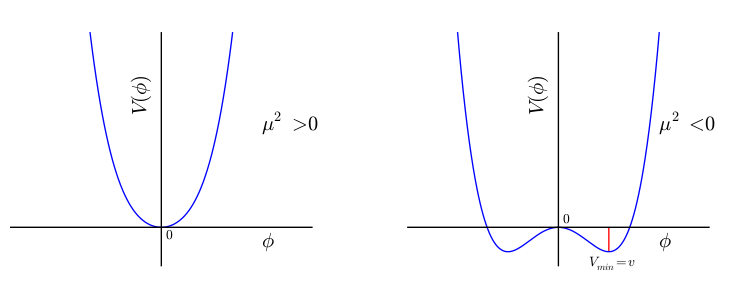
\includegraphics[width=13cm,height=5cm]{ch1/figures/HiggsPotential.png}
\caption{Example of electroweak symmetry breaking for the potential with real scalar, $V(\phi)=\mu^{2}\phi^{2} + \phi^{4}$. The ground state
for $\mu^{2}<0$ no longer respect the symmetry $\phi\to-\phi$.}
\label{fig:HiggsPotential}
\end{figure}

By chosing a particular ground state, the symmetry is broken spontaneously. As we need to keep the $U(1)$ symmetry of electromagnetism,
we choose the configuration where the expectation value of the charged Higgs-field vanishes, and ground state can be written as:
\begin{equation}
\Phi\equiv\langle\Phi_{0}\rangle=\frac{1}{\sqrt{2}}\left(\begin{array}{c} 0 \\ v \end{array}\right), \:\:\: v =\frac{\mu}{\sqrt{\lambda}}
\end{equation}
We have chosen $\phi_{3}=v$ and $\phi_{1}=\phi_{2}=\phi_{4}=0$, a direction in $SU(2)$ space. Now, considering a small perturbation to 
investigate the excitation of the field,
\begin{equation}
\Phi(x) = \frac{1}{\sqrt{2}} \left(\begin{array}{c} 0 \\ v + h(x) \end{array}\right)
\end{equation}
Using relations in \eqn{\ref{eq:AZ}} and \eqn{\ref{eq:CovDer}}, and solving for the kinetic term of the Lagrangian we get,
\begin{eqnarray}
|D_{\mu}\Phi|^{2} = \frac{1}{2}(\partial_{\mu}h)^{2}  + \frac{1}{4}g'^{2}(v+h)^{2}(W_{\mu}^{+}W^{\mu-}) + 
                    \frac{1}{8}(g^{2} + g'^{2})(v+h)^{2}Z_{\mu}Z^{\mu}
\end{eqnarray}
Finally, the Higgs mechanism breaks the symmetry, and generates the mass terms for the bosons weak field. The mass terms for the gauge bosons at 
the leading order sare:
\begin{equation}
m_{\gamma} = 0,\:\:\:m_{W^{\pm}} = \frac{vg}{2}, \:\:\:\text{and}\:\:\:m_{Z}=\frac{1}{2}v\sqrt{g^{2}+g'^{2}}
\end{equation}
where we have the relation $m_{W}/m_{Z}=\cos\theta_{W}$. A measurement of all the three parameters, mass of $W$, mass of $Z$ and
$\cos\theta_{W}$, allows the testing of SM predictions. We also get a real Goldstone boson, $h$, which is identified as the Higgs boson.

Plugging in the expansion around the $vev$ into the potention of the Lagrangian in \eqn{\ref{eq:HiggsLag}}, 
\begin{equation}
\mathcal{L} = -\lambda v^{2}h^{2} - \lambda v h^{3} - \frac{\lambda}{4}h^{4}
\end{equation}
leads to a three-point, four-point Higgs boson vertex, and mass term where, $m_{h}=\sqrt{2\lambda v^{2}}$. The parameter $\mu$ which
defines the Higgs boson mass cannot be predicted by the theory. The recently discovered new boson at the Large Hadron 
Collider~\cite{Chatrchyan:2012xdj,Aad:2012tfa}, which is a strong candidate for Higgs boson and has a mass of roughly 125\unit{GeV}, fixes the 
value of $\mu$. 

Fermionic mass terms can also be generated using the same complex scalar doublet by adding Yukawa couplings to the Higgs field in the Lagrangian:
\begin{equation}
\mathcal{L}_{Yukawa} = \sum_{f}^{\text{family}=1,2,3}\Big[ -y_{\ell}\bar{L}\Phi e_{R} - y_{d}\bar{Q}\Phi d_{R} 
                       - y_{u}\bar{Q}(-i\sigma_{2})\Phi^{\ast} u_{R} + h.c. \Big]
\end{equation}
%where $(-i\sigma_{2})\Phi^{\ast}$ is required to get the $vev$ aligned with the up-type quarks, 
where $u_{R}$, $d_{R}$ ($e_{R}$) are the quark (lepton) $SU(2)_{L}$ doublets and singlets. The constants $y_{\ell,d,u}$ are the free parameters of the 
model. After breaking the electroweak symmetry, these terms become:
\begin{equation}
\mathcal{L}_{Yukawa} = \sum_{f}^{\text{family}=1,2,3}\Big[  -\frac{1}{\sqrt{2}}y_{\ell}\bar{\ell}_{L}(v+h)\ell_{R}    
                                                            -\frac{1}{\sqrt{2}}y_{q}\bar{q}_{L}(v+h)q_{R}  \Big],
\end{equation}
such that the masses of the fermions are $m_{f} = y_{f}v/\sqrt{2}$. There are also terms with $h\bar{f}_{L}f_{R}$ interactions with coupling
strength proportional to the fermion masses.

\section{Beyond the Standard Model}
The SM of particle physics is one of the most successful theories in physics. It has passed all the tests and has been verified
experimentally with tremendous precision. One of its latest triumphs is the discovery of a new boson~\cite{Chatrchyan:2012xdj,Aad:2012tfa}, 
which to date appears to be the Higgs boson as predicted by the SM. Despite the success SM has achieved, there are reasons to believe that it is
far from the ultimate theory to explain the fundamental particles and their interactions. Some of the prominent issues that SM fail to address
and motivates physicist to look beyond are listed below :
\begin{itemize}
\item Neutrinos are treated as massless particles within the SM\footnote{$\nu_{R}$ are absent in Weinberg's paper~\cite{Weinberg:1967tq} as there was no 
evidence for neutrino mass by that time.}, but there have been experimental 
observations~\cite{Fukuda:1998mi,Fukuda:2001nk,Araki:2004mb,Michael:2006rx} which suggests that they do have a non-vanishing mass.

\item The SM gives no explanation for the large difference in the strength of fundamental forces. Also, the theory gives no reason for the wide 
range of masses for different SM particles. %Moreover, additional particles are required to cancel diverging loop-corrections to the Higgs mass. 
%\item  The SM gives no explanation for the large difference between the electroweak scale ($\mathcal{O}$(100\unit{GeV})), the scale of grand 
%unification, at which  electroweak and strong interactions becomes equally strong ($\mathcal{O}(10^{16}\unit{GeV})$), and the Planck scale 
%of $\mathcal{O}(10^{19}\unit{GeV})$, at which the gravitational force becomes as strong as the other forces.  

\item There is no explanation within the SM which may address the fact that there are three generations of fundamental fermions.
\item The SM does not explain the asymmetry between the matter and antimatter required to get all of the observed baryonic matter in the universe. 
%This require CP violation by an amount that can't be accomodated in the SM.

\item Finally, the cosmological and astrophysical observations concluded that the observed matter account for only about 5\% of the energy
and mass content of the universe. About 25\% is attributed to the non-luminous dark matter and the remaining 70\% are dark 
energy~\cite{Riess:1998cb}. None of these last two issues find any explanation within the SM.
%%~\cite{Ryabov:1900zz,Prakash2012,Chernin:2008zz}
\end{itemize}

\subsection{The Excited Quark Model}\label{Se:qstarTheory}
Physicists have come up with different ideas/models to address the questions that the standard model fails to answer. 
One of the directions which may shed light on some of these unanswered questions is the idea of quark compositeness, which suggests that 
quarks may not be fundamental particles but are composite entities of more fundamental particles (often referred to as ``preons'')~\cite{Pati:1975md,Eichten:1983hw,Baur:1987ga,Baur:1989kv}.
Simple motivation which makes us think towards this path comes from the historical developments, where we have always found something new when 
probed with higher energies. 

$\text{Matter}\to\text{Molecules}\to\text{Atom}\to\text{Nucleons}\to\text{quarks/leptons}\to\text{\bf What Next ???}$ \\
With the LHC\footnote{Large Hadron Collider, more details mentioned in Chapter~\ref{ch:ExptApp}} colliding protons at a center-of-mass energy 
of 8\unit{TeV}, the hunt for the more fundamental constituent if it exists, is still on.
The SM does not give any insight to the wide range of fermion masses nor does it explain the replication of fermion families, as stated in earlier 
section. This has led to the speculation that quarks and leptons are not elementary particles but are composite objects. If compositeness of 
fermion exists, it may also proffer to explain parameters like particle mass, charge, which the SM had failed to explain. 

The most compelling sign for substructure of quarks would be the discovery of an excited state of a quark, which we denote by \qstar.
To supplement the belief that compositeness would lead to an excited state, a simple analogy is considered. We know that the excited
states of known particles are common in nature, for example, the excited state of hydrogen atom. Hydrogen atom in its ground state absorbs
a photon and goes to its excited states. The excited hydrogen atom then radiates photons to reach to its ground state. Likewise, if quarks
have sub-structure, we expect them to exhibit excited states. A gluon interaction could excite a quark and while returning to ground state, 
they would radiate either a photon or a gluon. 

The preons, if exists, would experience an unknown force due to an asymptotically free but confining gauge interaction, which becomes very 
strong at a characteristic scale $\Lambda$ also referred to as compositeness scale, forming bound  states, that we see as quarks. Excited 
quarks may couple to ordinary quarks and leptons via contact interactions resulting from strong preon interactions for $\Lambda\gg\sqrt{\shat}$. 
For $\Lambda<\sqrt{\shat}$, excited quarks can be produced on-shell via gauge mediation. In this study, it is assumed that the LHC energy is 
larger than the compositeness scale, $\Lambda$ and excited quark states have a mass scale comparable to that of the dynamics of the new
binding force, i.e., $\mqstar=\Lambda$. While we expect $\mqstar \le \Lambda$, the equality has been assumed essentially to reduce the number
of unknown parameters.

The simplest excited quark model~\cite{Baur:1989kv} used in this study assumes the excited quarks to have both spin and isospin 1/2 and have
their left- and right-handed components in weak isodoublets.
%, e.g., for the first generation,
%\begin{equation}
%\left[ \begin{array}{c} u \\ d \end{array} \right]_{L} \; , \; 
%\begin{array}{c} u_{R} \\ d_{R} \end{array}
%\left[ \begin{array}{c} u^{\star} \\ d^{\star} \end{array} \right]_{L} \; , \; 
%\left[ \begin{array}{c} u^{\star} \\ d^{\star} \end{array} \right]_{R}
%\end{equation}
The coupling of excited quarks, $q^{\star}$ to gluons, $\gamma$, $W^{\pm}$ and $Z$ is vectorlike and is given by the Lagrangian~\cite{Baur:1989kv},
\begin{equation}
\mathcal{L}_{gauge} = \bar{q^{\star}}\gamma^{\mu} \left[ g_{s}\frac{\lambda^{a}}{2}G_{\mu}^{a} + g\frac{\tau}{2}W_{\mu} + g'\frac{Y}{2}B_{\mu} \right]q^{\star}
\end{equation}
where, $g_{s}$, $g=\frac{e}{\text{sin}\theta_{W}}$ and $g'=\frac{e}{\text{cos}\theta_{W}}$ are the strong and electroweak gauge coupling constants; 
$G_{\mu}^{a}$, $W_{\mu}$, $B_{\mu}$ describe the gluon, $SU(2)$, and $U(1)$ gauge fields; $Y$ is the weak hypercharge of excited states of quark 
with a value of 1/3. Assuming the mass of excited quarks to be of the order of $\Lambda$, the transition between the excited state (right-handed)
and the ground state (left-handed) of quarks is constrained by gauge invariance and is given by an effective Lagrangian of the magnetic-moment type, 
\begin{equation}
{\mathcal L}_{int} = \frac{1}{2\,\Lambda}\bar{q^{\ast}_{R}} \, \sigma^{\mu\nu}
\left[g_{s}f_{s}\frac{\lambda_{a}}{2}G^{a}_{\mu\nu}\;+\;gf\frac{\tau}{2}W_{\mu\nu}\;+\;g'f'\frac{Y}{2}B_{\mu\nu} \right] q_{L} + h.c.,
\label{eq:Lagrangian1}
\end{equation}
where $G^{a}_{\mu\nu}$, $W_{\mu\nu}$ and $B_{\mu\nu}$ are the field-strength tensors of the SU(3), SU(2) and U(1) gauge fields, respectively.
The quantities $\lambda_{a}$, $\tau$, $Y$ ($g_{s}$, $g$, $g'$) are the corresponding generators (gauge coupling constants). 
$\Lambda$ denotes the typical scale of these interactions. The unknown dimensionless constants $f_{s}$, $f$, $f'$ are determined by the 
dynamics of compositeness and are assumed to be of order unity.

In proton-proton collisions, excited quarks could be produced at the tree level predominantly by quark gluon scattering(\fig{\ref{fig:qstarS}}), 
and then by quark anti-quark annihilation~(\fig{\ref{fig:qstarT}}). At the loop level, they would show their presence in gluon gluon 
fusion~(\fig{\ref{fig:qstarBox}}). %The loop level contribution is not considered in the study as it would make the effective theory
%non-renormalizable. Non-renormalizability can be cured by introducing suitable higher dimension operators but then the contribution would
%presumably be significantly low as compared to the tree level diagrams to have any meaningful effect on our analysis. 
The loop level diagram is not considered in the study as its contribution would presumably be significantly smaller as compared to the tree level diagrams to have any meaningful effect on our analysis.
\begin{figure}[!h]
%\vspace{-1.5cm}
\centering
 \subfloat[quark gluon fusion]{\label{fig:qstarS}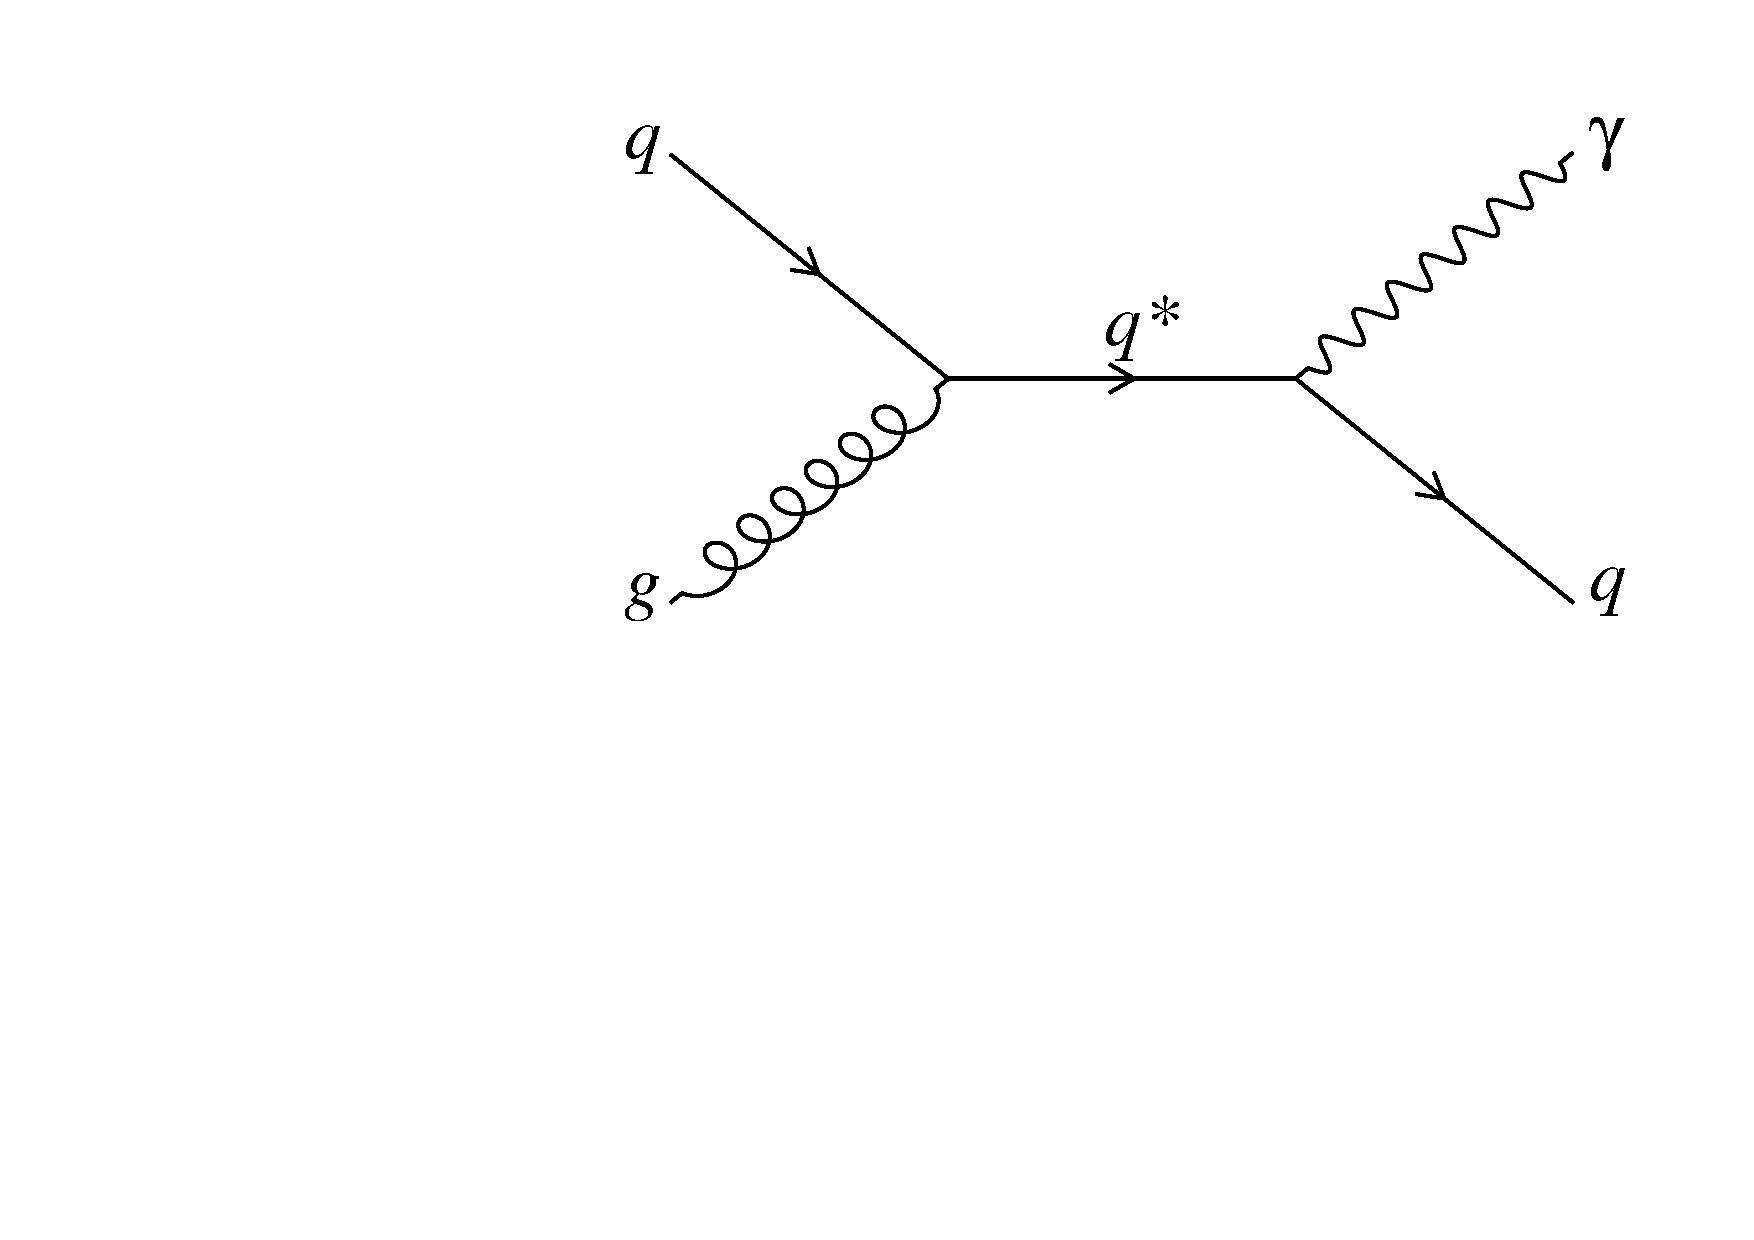
\includegraphics[width=5cm,height=4.cm]{ch1/figures/qgQstarqgamma_S.pdf}}
 \subfloat[quark anti-quark annihilation]{\label{fig:qstarT}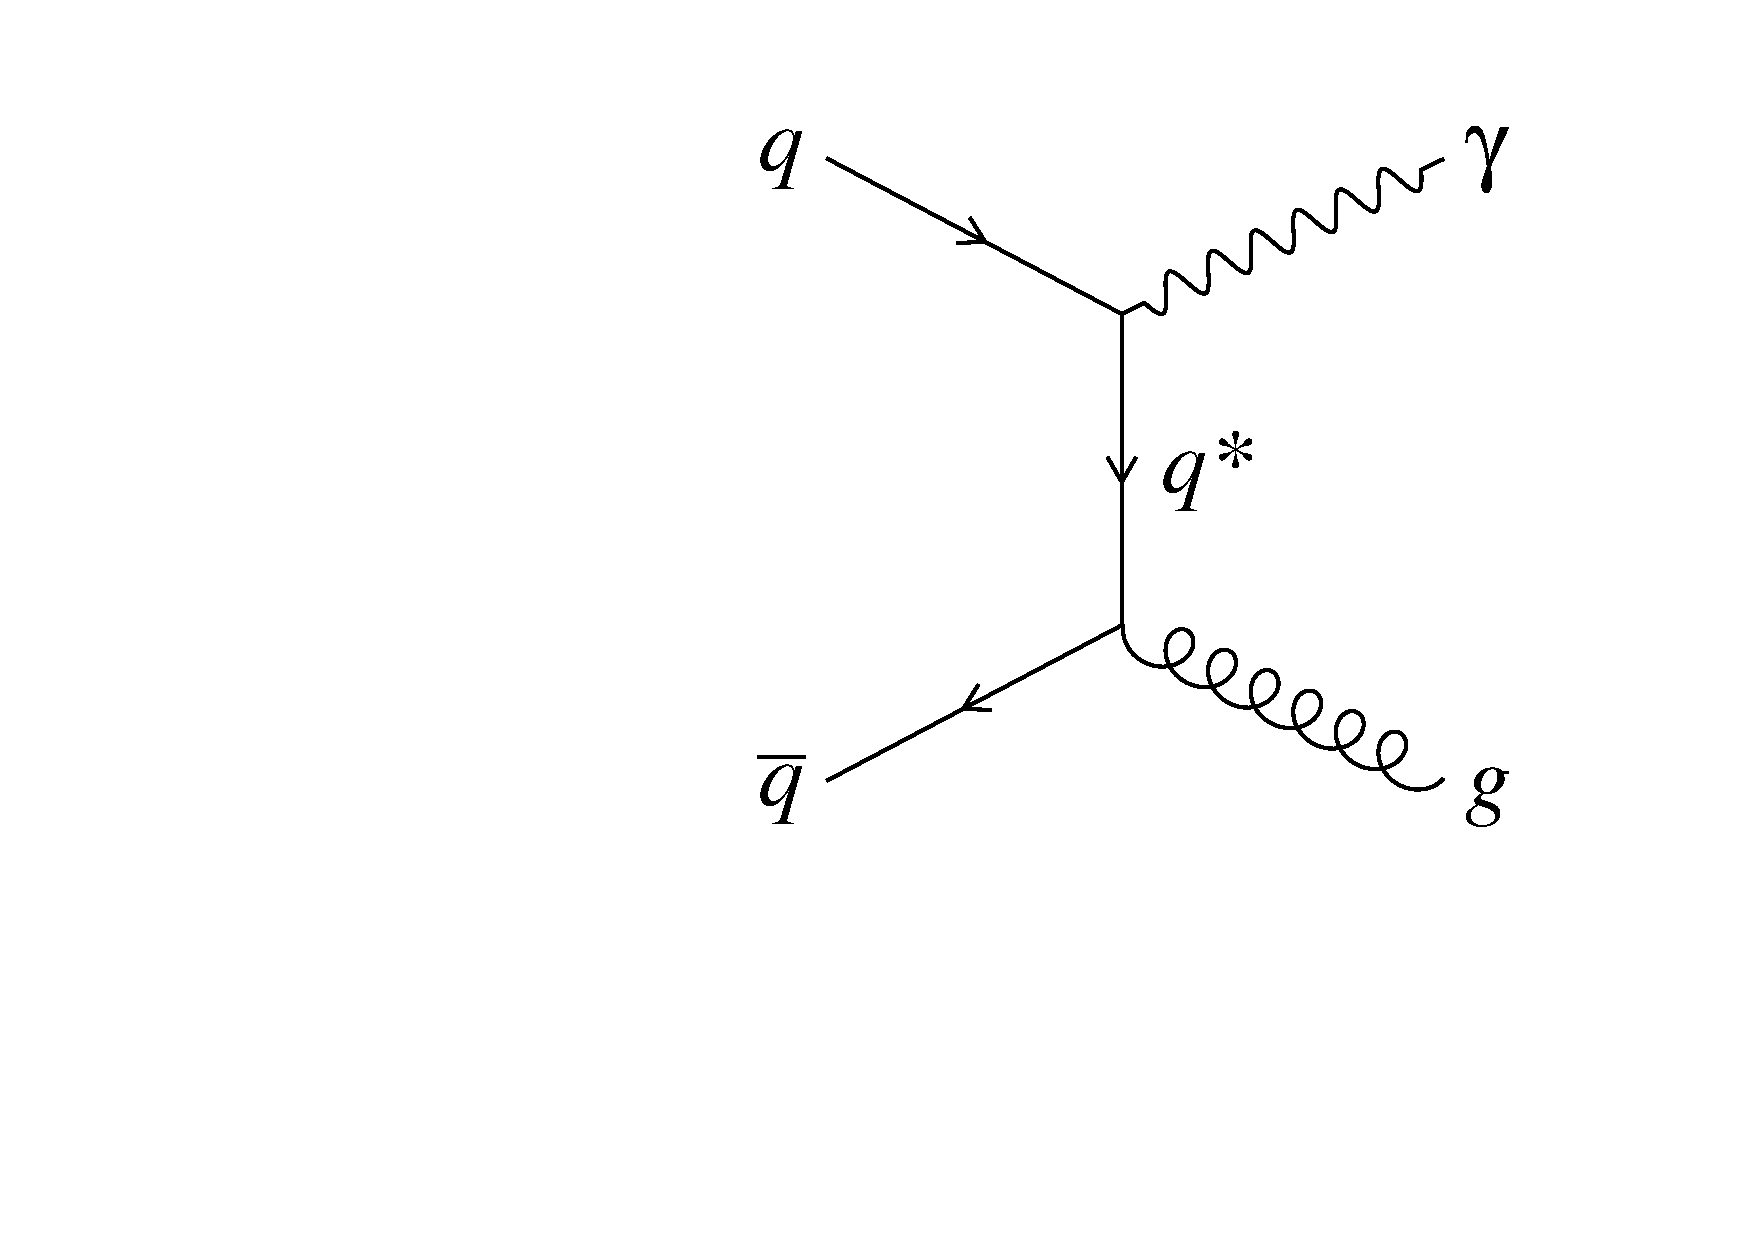
\includegraphics[width=6cm,height=4cm]{ch1/figures/qqbarQstarggamma_T.pdf}}
 \subfloat[gluon gluon fusion]{\label{fig:qstarBox}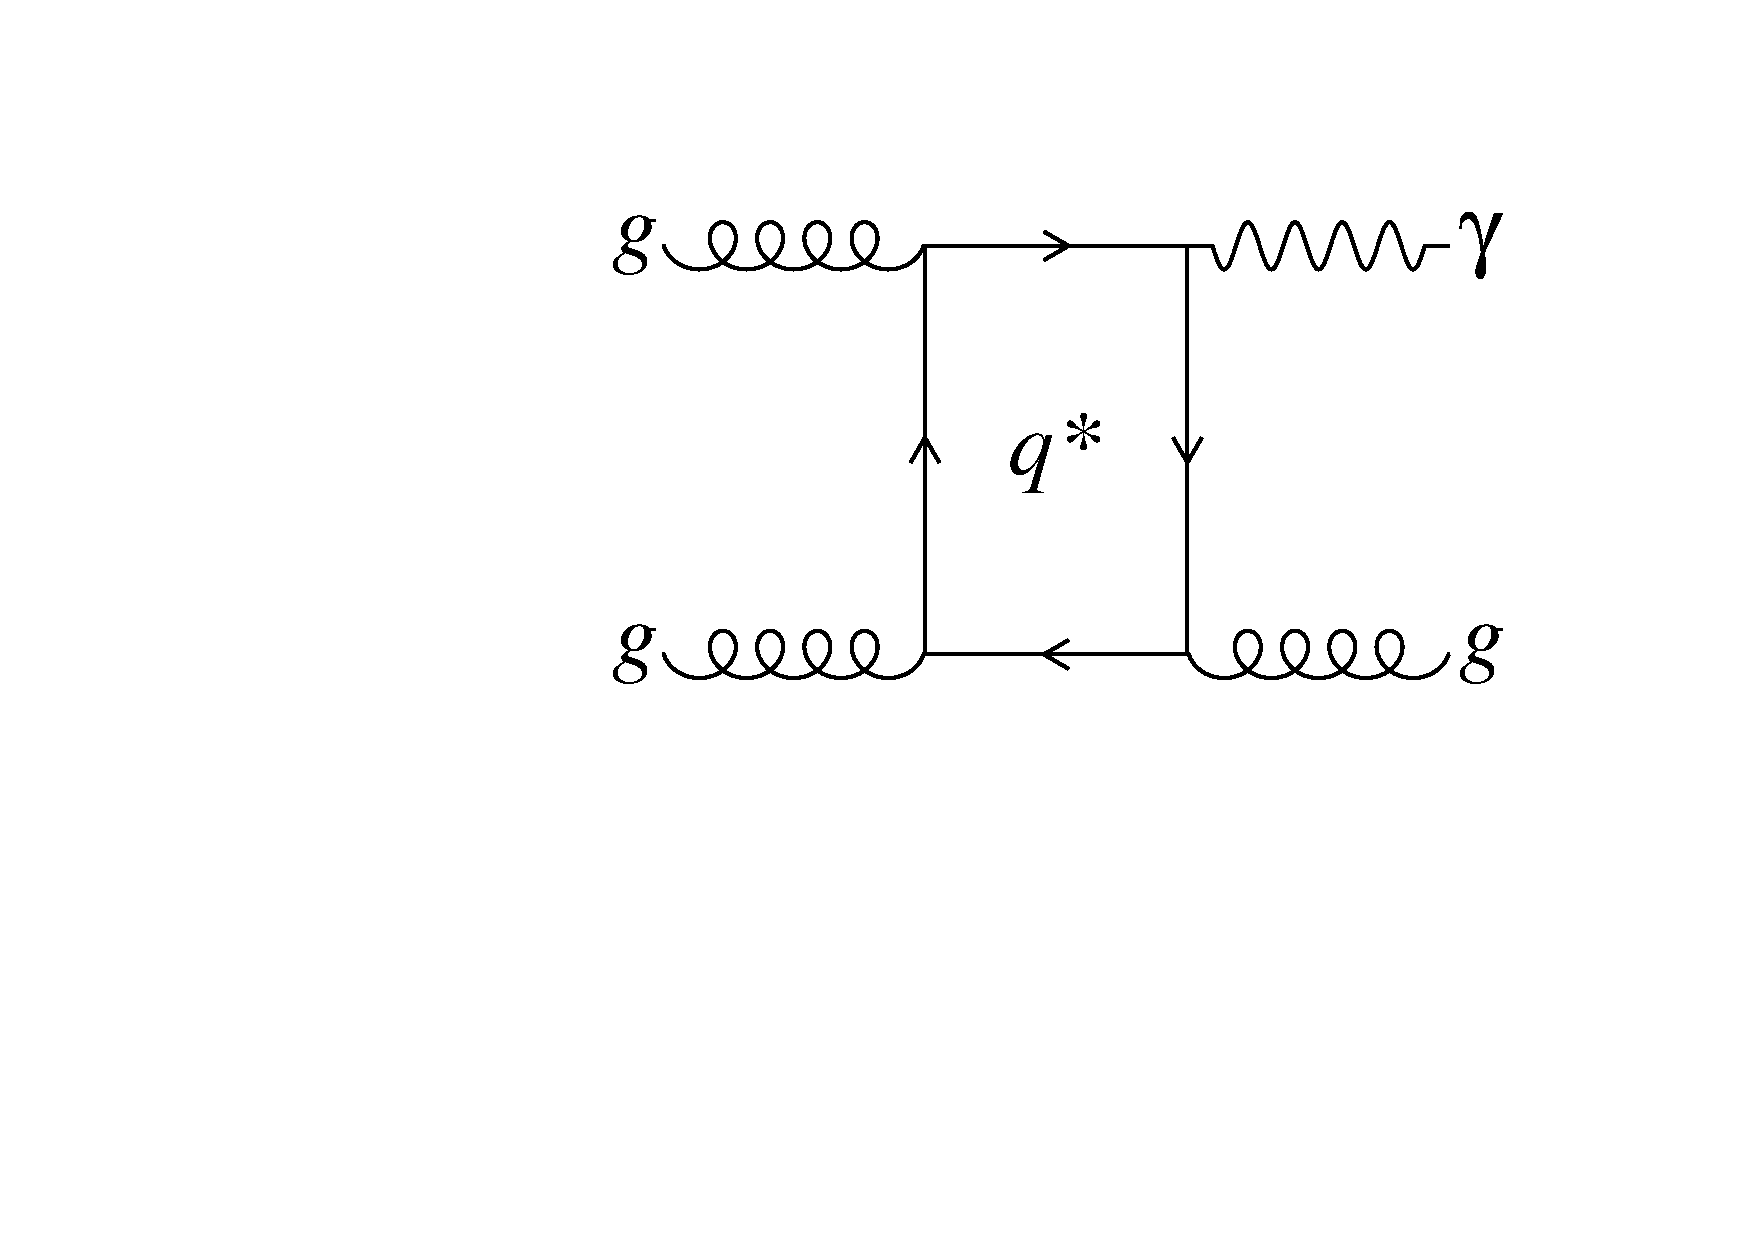
\includegraphics[width=6cm,height=4cm]{ch1/figures/ggQstargg.pdf}}
 \caption{Some of the Feynman diagrams for $pp\rightarrow\qstar\rightarrow$ \gamjet final state.}
\label{fig:qstarSig}
%\vspace{-1cm}
\end{figure}
The excited quark \qstar then decays into a ground-state quark and a gauge boson ($g$, W, Z, $\gamma$). Using \eqn{\ref{eq:Lagrangian1}}, assuming 
$\mqstar > {\mathrm M_{V}}$ ($V=W^{\pm},Z^{0}$) and neglecting the ground-state quark masses, the partial widths for various channels are given by,
\begin{eqnarray}
\Gamma(q^{\star}\to{qg})  & = & \frac{1}{3}\alpha_{s}f_{s}^{2}\frac{M_{q^{\star}}^{2}}{\Lambda^{2}}, \\
\Gamma(q^{\star}\to{q\gamma}) & = &\frac{1}{4}\alpha f_{\gamma}^{2}\frac{M_{q^{\star}}^{3}}{\Lambda^{2}}, \\
\Gamma(q^{\star}\to{qV}) & = &\frac{1}{8}\frac{g^{2}_{V}}{4\pi}f_{V}^{2}\frac{M_{q^{\star}}^{3}}{\Lambda^{2}}
      \left(1-\frac{M^{2}_{V}}{M^{2}_{q^{\star}}}\right)\left(2+\frac{M^{2}_{V}}{M^{2}_{q^{\star}}}\right),
\end{eqnarray}
with
\begin{eqnarray}
f_{\gamma} & = & fT_{3}+f'\frac{Y}{2}, \\
f_{Z} & = & fT_{3}\text{cos}^{2}\theta_{W} - f'\frac{Y}{2}\text{sin}^{2}\theta_{W}, \\
f_{W} & = & \frac{f}{\sqrt{2}}
\end{eqnarray}
where $T_{3}$ is the third component of the weak isospin. Setting the compositeness scale $\Lambda$ to be the \qstar mass and assuming the SM coupling, 
\ie, $\Lambda=\mqstar$ and $f_{s}=f=f'=1$, \tab{\ref{Table:qstarBR}} shows the numerical values of the relative branching ratios of the \qstar. The 
\qstar final states are large transverse momentum jet$-$jet, $\gamma-$jet, $Z^{0}-$jet
or $W^{\pm}-$jet pairs. 
%---------------TABLE FOR MC samples-------------------
\begin{table}[h!]
\begin{center}
%\begin{ruledtabular} 
%\resizebox{16cm}{!}{
\begin{tabular}{l|l||l|l}
\hline
\hline
 Decay Channel       & BR     & Decay Channel        & BR \\
\hline
$\ustar\to$ug        & 83.4\% & $\dstar\to$dg        & 83.4\% \\
$\ustar\to$u$\gamma$ & 2.27\% & $\dstar\to$d$\gamma$ & 0.57\% \\
$\ustar\to$u$Z^{0}$  & 3.39\% & $\dstar\to$d$Z^{0}$  & 5.07\% \\
$\ustar\to$d$W^{-}$  & 10.9\% & $\dstar\to$u$W^{+}$  & 10.9\% \\
\hline
\end{tabular}
%}
\caption{The branching ratios (BR) of various decay channels of the \qstar (\ustar, \dstar) of mass $\mqstar=1\unit{TeV}$.}
%\end{ruledtabular}
   \label{Table:qstarBR}
\end{center}
\end{table}


In this study, we present a search for excited quark in the photon + jet final state. An encouraging fact for the present work is that the 
background processes for $\qstar\to\gamjet$ are well understood both theoretically as well as experimentally. It is assumed throughout 
the study that the compositeness scale $\Lambda$ is less than the LHC center-of-mass energy and gauge interactions dominate over contact interactions. 
For $\Lambda$ smaller than the LHC center-of-mass energy, excited quarks are produced dominantly through s-channel processes. The s-channel quark 
gluon scattering of excited quarks would give a resonance over the SM continumm in the \gamjet invariant mass distribution peaking at 
M$_{\gamma j}=\mqstar$ while all other modes would give excess of events over the continuum prediction. The SM result will be recovered in the 
limit $\Lambda\to\infty$ which also implies that higher the compositeness scale $\Lambda$, harder it is to observe the signal for new physics. 

\subsubsection{A Summary of Previous Searches}
Searches for quark compositeness have been performed by various experiments of different generations at different energies
and in several decay channels with no success. A summary of results from these experiments is reported in this section.

The ZEUS detector at the \gls{HERA} experiment searched for heavy excited states of quarks in $e^{+}p$ collisions at a center-of-mass
energy of 300\unit{GeV} with an integrated luminosity of 9.4\pbinv and excluded, at 95\% confidence level, excited quarks with mass between 40 
and 169\unit{GeV}~\cite{Breitweg:1997qa}. The H1 detector at the same experiment also performed searches in various decay channels, but with a 
lower integrated luminosity (37\pbinv) and reported the results in Ref.~\cite{Tome:966798}. 
%\begin{figure}[h]
%\centering
%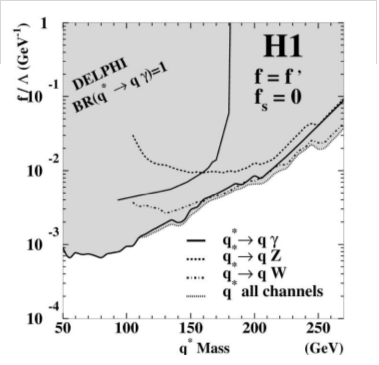
\includegraphics[width=8cm,height=6cm]{ch1/figures/H1_HERA_Limits.png}
%\caption{Upper limits on the couplings $f/\Lambda$ at 95\% confidence level as a function of the mass for the excited quark seacrh in H1 
%experiments at HERA.}
%\label{fig:H1_Limits}
%\end{figure}

The CDF collaboration at the Tevatron experiment searched for excited quarks in the \gamjet and dijet decay channels 
in $p\bar{p}$ collisions at $\sqrt{s}$ = 1.8 TeV and excluded the mass range of $80<\mqstar<540\unit{GeV}$~\cite{CDFexclgj}
and $200<\mqstar<520\unit{GeV}$ \nd $580<\mqstar<760\unit{GeV}$~\cite{CDFexcljj}, respectively, with 95\% confidence level.
The D0 collaboration at the Tevatron experiment searched in the dijet final state only~\cite{D0excl} and excluded masses 
 below 775\unit{GeV} at 95\% confidence level. The ATLAS collaboration at the LHC experiment excluded excited 
quarks below 4.06\unit{TeV} with 95\% confidence level in the dijet decay channel~\cite{Aad:2014aqa} in $pp$ collisions at 
$\sqrt{s}$ = 8\unit{TeV} and below 3.5\unit{TeV} in the \gamjet decay channel~\cite{Aad:2013cva}.
The CMS collaboration at the LHC experiment has also excluded excited quarks below 3.19\unit{TeV} in the dijet final state with 95\% CL 
in $pp$ collisions at $\sqrt{s}$ = 8\unit{TeV}~\cite{CMSexcl8jj}. 
